\chapter{Terrain Classification for hexapod robot AMOS II} \label{chap:terrain_classification}

The classification problem in this thesis relates to AMOS II, an open-source multi sensori-motor robotic platform (see \cref{img:amosii}). The task is to classify various terrain types based on proprioceptive (joint angles) and tactile (ground contact) sensors. The overall process is based on simulation data and as stated in \cref{chap:kitt_nn}, feedforward neural networks are used for classification.

\section{Overall Process Summary} \label{sec:overall_process_summary}
The overall process consists of several modules. The workflow is illustrated in \cref{img:terrain_overall_simple} (a more detailed diagram can be found in \cref{img:app:terrain_classification_process}).

\begin{figure}[H]
  \centering
  \includegraphics[width=0.5\textwidth]{terrains_overall_simple.png}
  \caption{Terrain Classification: overall process diagram}
  \label{img:terrain_overall_simple}
\end{figure}

The very first step is to make the AMOS II simulation run (\cref{ssec:lpzrobots_sim}). Then a simple tripod gait controller is implemented (\cref{ssec:tripod_gait_controller}). To generate various terrain types, the number of variable terrain quailities and their ranges are determined (\cref{ssec:terrain_qualities}). Based on these qualities (parameters), a number of virtual terrains is defined (\cref{ssec:terrain_parameters}) and an optimality of these parameters is briefly analysed (\cref{ssec:terrains_analysis}).

Next, AMOS II (its simulation alternative) is forced to walk on every defined terrain type several times and for a sufficiently long period of time and the data from all proprioceptors are saved. This data is then verified and failing experiments are removed. The data acquisition step is parameterized by a standard deviation of an additive (Guassian) terrain noise and is run for several values.

Having the clean simulation data from all sensors, a feature vector structure is determined. Then a Gaussian signal noise is added. 

Finally, a dataset is created by splitting all the data into training, validation and testing sets. As it is indicated in \cref{img:app:terrain_classification_process}, several datesets and several classifiers are generated during the process. 

The dataset packages may differ in these parameters:
\begin{itemize}
\item terrain types included (-> number of classes)
\item sensors on input
\item samples length (number of simulation timesteps)
\item terrain noise and signal noise
\item number of samples
\end{itemize}

The trained networks may differ in the following parameters:
\begin{itemize}
\item dataset that the network has been tested on
\item neural network structure, learning rate and number of epochs
\end{itemize}

An optimal neural network classifier is found. The optimal network is then pruned by the algorithm developed in \cref{sec:network_pruning_algorithm}. The classification performance of developed tools is compared to \textit{Scikitlearn-neuralnetwork} classification library \citep{misc:sknn}.

\section{Experimental Environment Specification}
The ultimate goal is to implement an online terrain classifier for selection of optimal walking gait on real hexapod robot AMOS II. Therefore the real robot is presented in the following section \ref{ssec:amosii}.

However, as already stated above, the proposed approach will be evaluated using simulated robot in a virtual environment. In this case, \textit{LPZ Robots simulator} \citep{misc:lpzrobots} was used and a description is given in section 6.2.2.

\subsection{Hexapod Robot AMOS II} \label{ssec:amosii}
The \textit{AMOS II} abbreviation stands for Advanced Mobility Sensor Driven-Walking Device - version II \citep{misc:amosii}. It is a biologically inspired hardware platform of size 30x40x20 cm and weight 5.8 Kg (see \cref{img:amosii}). It is mainly used to study a neural control, memory and learning for machines with many degrees of freedom. The body and parts of the robot are inspired by a cockroach.

\begin{figure}[H]
  \centering
  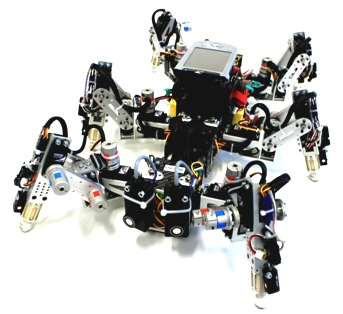
\includegraphics[width=343px]{amosii}
  \caption{AMOS II. \citep{misc:amosii}}
  \label{img:amosii}
\end{figure}

A wide range of sensors (for instance infra-red, reflexive optical, light-dependent, laser, camera, inclinometer sensors) allows AMOS II to perform several kinds of autonomous behaviour including foothold searching, elevator reflex (swinging a leg over obstacles), self-protective reflex (standing in an upside-down position), obstacle avoidance, escape responses etc. \citep{misc:amosii}. However, only proprioceptive and tactile sensors are important for this study. Therefore, we focus on joint angle sensors and foot contact sensors. All of them are located on robot's legs. The leg structure is shown in \cref{img:amosii_leg}.

\begin{figure}[H]
  \centering
  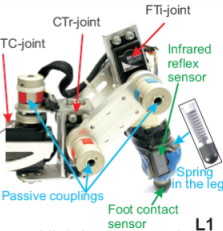
\includegraphics[width=0.5\textwidth]{amosii_leg}
  \caption{Structure of the AMOS's leg. \citep{misc:amosii}}
  \label{img:amosii_leg}
\end{figure}

As shown in \cref{img:amosii} and \cref{img:amosii_leg}, the robot has \textit{6 foot contact sensors} in total, one on each leg. Each of them returns a value from range $ [0.0, 1.0] $ depending on how strong the foot contact is, i.e., it is equal $ 1.0 $ if the robot stands on the leg with its full weight and it equals $ 0.0 $ when the leg is in the air.

There are three joints on each of the robot's legs. The thoraco-coxal (TC-) joint is responsible for forward/backward movements. The coxa-trochanteral (CTr-) joint enables elevation and depression of the leg and the last one, femur-tibia (FTi-) joint is used for extension and flexion of the tibia.

These joints are physically actuated by standard servo motors. Angles of the joints are measured by the servo motors and are considered as propriceptive sensors. As AMOS II has six legs and there are three joints on each leg, there are \textit{18 angle sensors} in total. There is also one backbone joint angle, however, as this one is not implemented in the simulation (see \cref{ssec:lpzrobots_sim}), it is omitted in this work.

In \cref{tab:proprioceptors} all the propriceptive sensors, their abbreviations and original ranges are listed. The ranges are based on the individual servo motors locations and are manually set to avoid collisions. In \cref{sec:feature_vector_compilation} a normalization of these ranges is discussed.

Robot actuators (servo motors) can generate movements of variable compliance by utilizing a virtual muscle model (see \cite{misc:amosii} for details). 

\begin{table}[H]
\centering
\caption{Summary of proprioceptive sensors of AMOS II hexapod robot}
\label{tab:proprioceptors}
\begin{tabular}{|l|l|c|}
\hline
\textit{abbr.} & \multicolumn{1}{c|}{\textit{sensor description}} & \textit{original range} \\ \hline
\textbf{ATRf}         & Angle sensor, Thoraco joint, Right front leg     & {[}-1.5, 1.5{]}         \\ \hline
\textbf{ATRm}         & Angle sensor, Thoraco joint, Right middle leg    & {[}-1.5, 1.5{]}         \\ \hline
\textbf{ATRh}         & Angle sensor, Thoraco joint, Right hind leg      & {[}-1.5, 1.5{]}         \\ \hline
\textbf{ATLf}         & Angle sensor, Thoraco joint, Left front leg      & {[}-1.5, 1.5{]}         \\ \hline
\textbf{ATLm}         & Angle sensor, Thoraco joint, Left middle leg     & {[}-1.5, 1.5{]}         \\ \hline
\textbf{ATLh}         & Angle sensor, Thoraco joint, Left hind leg       & {[}-1.5, 1.5{]}         \\ \hline
\textbf{ACRf}         & Angle sensor, Coxa joint, Right front leg        & {[}-1.5, 1.5{]}         \\ \hline
\textbf{ACRm}         & Angle sensor, Coxa joint, Right middle leg       & {[}-1.5, 1.5{]}         \\ \hline
\textbf{ACRh}         & Angle sensor, Coxa joint, Right hind leg         & {[}-1.5, 1.5{]}         \\ \hline
\textbf{ACLf}         & Angle sensor, Coxa joint, Left front leg         & {[}-1.5, 1.5{]}         \\ \hline
\textbf{ACLm}         & Angle sensor, Coxa joint, Left middle leg        & {[}-1.5, 1.5{]}         \\ \hline
\textbf{ACLh}         & Angle sensor, Coxa joint, Left hind leg          & {[}-1.5, 1.5{]}         \\ \hline
\textbf{AFRf}         & Angle sensor, Femur joint, Right front leg       & {[}-1.5, 1.5{]}         \\ \hline
\textbf{AFRm}         & Angle sensor, Femur joint, Right middle leg      & {[}-1.5, 1.5{]}         \\ \hline
\textbf{AFRh}         & Angle sensor, Femur joint, Right hind leg        & {[}-1.5, 1.5{]}         \\ \hline
\textbf{AFLf}         & Angle sensor, Femur joint, Left front leg        & {[}-1.5, 1.5{]}         \\ \hline
\textbf{AFLm}         & Angle sensor, Femur joint, Left middle leg       & {[}-1.5, 1.5{]}         \\ \hline
\textbf{AFLh}         & Angle sensor, Femur joint, Left hind leg         & {[}-1.5, 1.5{]}         \\ \hline
\textbf{FRf}          & Foot contact sensor, Right front leg             & {[}0.0, 1.0{]}          \\ \hline
\textbf{FRm}          & Foot contact sensor, Right middle leg            & {[}0.0, 1.0{]}          \\ \hline
\textbf{FRh}          & Foot contact sensor, Right hind leg              & {[}0.0, 1.0{]}          \\ \hline
\textbf{FLf}          & Foot contact sensor, Left front leg              & {[}0.0, 1.0{]}          \\ \hline
\textbf{FLm}          & Foot contact sensor, Left middle leg             & {[}0.0, 1.0{]}          \\ \hline
\textbf{FLh}          & Foot contact sensor, Left hind leg               & {[}0.0, 1.0{]}          \\ \hline
\end{tabular}
\end{table}

It is possible to generate various gaits using joint actuators and robot's neural locomotion control. The gait controller used to generate robot locomotion is described in \cref{ssec:tripod_gait_controller}.

\subsection{AMOS II Simulation} \label{ssec:amosii_sim}
The \textit{lpzrobots} project, developed by a research group at the University of Leipzig \citep{misc:lpzrobots} under GPL license, is used for AMOS II virtual representation. Some implementation details are discussed in \cref{ssec:app:lpzrobots_sim}. The project modules important for this study are shown in \cref{img:lpzrobots_repos}.

With reference to \cref{app:code_documentation}, the \textit{main.cpp} file from \path{root/simulation/mbulinai22015-gorobots_edu-fork/practices/amosii} directory can be called as the main simulation file for purposes of the thesis. It sets up the environment with initial parameters:

\begin{itemize}
\item $ controlinterval = 10 $
\item $ simstepsize = 0.01 $
\end{itemize}

This results in setting the simulation sensitivity to \textit{10 steps} per second.

\begin{figure}[H]
  \centering
  \includegraphics[width=1.0\textwidth]{lpzrobots_repos}
  \caption{Structure of the two repositories: LPZRobots and GoRobots. \citep{misc:lpzrobots}}
  \label{img:lpzrobots_repos}
\end{figure}

The initial robot position in the map is chosen randomly in order to generate a different route everytime the simulation is launched. The robot fixator, which is originally implemented for AMOS II, is removed, so the robot starts walking right after the simulation is launched.

The \textit{main.cpp} file contains all terrain types parameters introduced in \cref{sec:virtual_terrain_types}. The required terrain to be simulated is then passed to this file as an argument. Additionally, the standard deviation value of Gaussian terrain noise (details in \cref{ssec:terrain_noise}) is set as another argument. 

Finally, the file is ready to take one more argument, which is a simulation noise represented by a float number. In this study it is fixed to zero though and only the terrain noise combined with a signal noise is used.

The virtual vizualization of AMOS II is illustrated in \cref{img:amosii_sim}.

\begin{figure}[H]
  \centering
  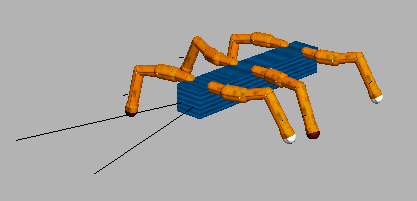
\includegraphics[width=0.8\textwidth]{amosii_sim}
  \caption{Virtual alternative for AMOS II.}
  \label{img:amosii_sim}
\end{figure}

Besides the backbone joint, all AMOS II actuators, proprioceptive and tactile sensors are modeled in the simulation and \textit{LpzRobots} framework is considered to provide an accurate simulated model of AMOS II.

\subsection{Tripod Gait Controller} \label{ssec:tripod_gait_controller}
The main motivation for the terrain classification is to adjust the current robot's gait accordingly and this way save some energy. In this work a \textit{tripod} gait (three legsg touching ground when walking) is used for classification. The tripod pattern is the fastest and most common gait for hexapods.

To generate the tripod gait, a central pattern generator (CPG) is used \citep{unpub:ai3_lec3}. It is implemented as a 2-neuron neural network as shown in \cref{img:two_neuron_network}.

\begin{figure}[H]
  \centering
  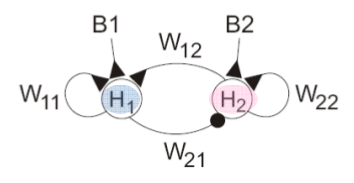
\includegraphics[width=0.5\textwidth]{two_neuron_network}
  \caption{2-neuron network oscillator \citep{unpub:ai3_lec3}}
  \label{img:two_neuron_network}
\end{figure}

The initial conditions and parameters of the implemented controller are shown in \cref{tab:tripod_controller_init}.

\begin{table}[H]
\centering
\caption{Initialization of \textit{tripod\_controller.h} (see \cref{app:code_documentation})}
\label{tab:tripod_controller_init}
\begin{tabular}{|l|c|l|}
\hline
\multicolumn{1}{|c|}{\textit{parameter}} & \textit{initial value} & \multicolumn{1}{c|}{\textit{description}} \\ \hline
$ aH_1 $                            & 0.0                    & activity of neuron $ H_1 $                     \\ \hline
$ aH_2 $                            & 0.0                    & activity of neuron $ H_2 $                     \\ \hline
$ oH_1 $                            & 0.001                  & output of neuron $ H_1 $                       \\ \hline
$ oH_2 $                            & 0.001                  & output of neuron $ H_2 $                       \\ \hline
$ bH_1 $                            & 0.0                    & bias for neuron $ H_1 $                        \\ \hline
$ bH_2 $                             & 0.0                    & bias for neuron $ H_2 $                        \\ \hline
$ wH_1H_1 $                          & 1.4                    & weight of the synapse from $ H_1 $ to $ H_1 $       \\ \hline
$ wH_1H_2 $                          & 0.4                    & weight of the synapse from $ H_2 $ to $ H_1 $       \\ \hline
$ wH_2H_1 $                          & -0.4                   & weight of the synapse from $ H_1 $ to $ H_2 $       \\ \hline
$ wH_2H_2 $                           & 1.4                    & weight of the synapse from $ H_2 $ to $ H_2 $       \\ \hline
$ p_1 $                              & 0.35                   & parameter for Thoraco joints              \\ \hline
$ p_2 $                              & 0.3                    & parameter for Coxa joints                 \\ \hline
\end{tabular}
\end{table}

Then, during the simulation, robot's joints are controlled in every simulation step by performing three actions:

\begin{enumerate}
\item \textbf{The activation function application}
\begin{equation}
a_i(t+1) = \displaystyle\sum_{j=1}^{n} w_{ij}o_j(t) + b_i, i = 1, ..., n
\end{equation}

\item \textbf{The transfer function application}
\begin{equation}
f(a_i) = tanh(a_i) = \frac{2}{1+e^{-2a_i}} - 1
\end{equation}

\item \textbf{Joint settings}

With the reference to previous equations and variables names, the actuators are set as shown in \cref{img:tripod_illustration}. The \textit{femur} joints (red ones) stay unchanged (set to zero). This setting generates a tripod gait for AMOS II.

\begin{figure}[H]
  \centering
  \includegraphics[width=200px]{tripod_illustration}
  \caption{Schematic diagram of tripod gait controller}
  \label{img:tripod_illustration}
\end{figure}
\end{enumerate}

\section{Generation of Virtual Terrains} \label{sec:generation_of_virtual_terrains}
Since the verification is based on the simulation only, the goal is to design a virtual environment. For this purpose various terrain types need to be virtually simulated.

A terrain is defined by four parameters: \textit{roughness}, \textit{slipperiness}, \textit{hardness} and \textit{elasticity}. These parameters form a substance together (this process is described in \cref{ssec:app:terrain_construction_in_main.cpp}).

Besides these four parameters represented as a substance handle, a terrain constructor takes six more arguments (used in \cref{code:terrain_ground}):

\begin{description}
\item[terrain\_color] : simulation ground color
\item["rough1.ppm"] : an image in the .ppm format, a lowest common denominator color image file format \citep{misc:ppm}, a bitmap height file
\item[""] : texture image (not used)
\item[20] : walking area x-size 
\item[25] : walking area y-size
\item[terrain\_height] : maximum terrain height
\end{description}

\subsection{Terrain Features} \label{ssec:terrain_features}
Out of the listed ground parameters, some of them are picked up and being called \textit{terrain features}, as they define a specific terrain type.

Therefore, a virtual terrain type is defined by five features. Each of them is a float number from an empirically stated range \footnote{The upper range limits have been set up based on significant changes in the robot behaviour for various parameter values.}. (\cref{tab:terrain_features}).

\begin{table}[H]
\centering
\caption{Terrain features and their ranges}
\label{tab:terrain_features}
\begin{tabular}{|l|c|c|c|c|} \hline
             & min value & min meaning & max value & max meaning \\\hline
roughness    & 0.0       & smooth		& 10.0		& rough     \\\hline
slipperiness & 0.0       & friction		& 100.0		& slippy    \\\hline
hardness     & 0.0       & soft			& 100.0		& hard	    \\\hline
elasticity   & 0.0       & rigid		& 2.0		& elastic   \\\hline
height       & 0.0       & low			& 0.1		& high		 \\\hline
\end{tabular}
\end{table}

\subsection{Features Determination for Various Terrains} \label{ssec:features_determination}
To determine a terrain type, one has to come up with the five parameters from \cref{tab:terrain_features}.

In this work we use 14 terrain types. Their parameters (shown in \cref{tab:terrains_parameters}) have been set up manually. With respect to the feature ranges from \cref{tab:terrain_features}, the values have been normalized between 0 and 1.

\begin{table}[H]
\centering
\caption{Parameters of virtual terrain types}
\label{tab:terrains_parameters}
\begin{tabular}{|l|l|c|c|c|c|c|}
\hline
\textit{\#}                                       & \textit{terrain title} & \multicolumn{1}{l|}{\textit{roughness}} & \multicolumn{1}{l|}{\textit{slipperiness}} & \multicolumn{1}{l|}{\textit{hardness}} & \multicolumn{1}{l|}{\textit{elasticity}} & \multicolumn{1}{l|}{\textit{height}} \\ \hline
1                         & \textbf{carpet}        & 0.3                                     & 0.0                                        & 0.4                                    & 0.15                                     & 0.2                                  \\ \hline
2                         & \textbf{concrete}      & 1.0                                     & 0.0                                        & 1.0                                    & 0.0                                      & 0.0                                  \\ \hline
3                         & \textbf{foam}          & 0.5                                     & 0.0                                        & 0.0                                    & 1.0                                      & 0.7                                  \\ \hline
4                         & \textbf{grass}         & 0.5                                     & 0.0                                        & 0.3                                    & 0.3                                      & 0.5                                  \\ \hline
5                         & \textbf{gravel}        & 0.7                                     & 0.001                                      & 1.0                                    & 0.0                                      & 0.3                                  \\ \hline
6                         & \textbf{ice}           & 0.0                                     & 1.0                                        & 1.0                                    & 0.0                                      & 0.0                                  \\ \hline
7                         & \textbf{mud}           & 0.05                                    & 0.05                                       & 0.005                                  & 0.25                                     & 0.2                                  \\ \hline
8                         & \textbf{plastic}       & 0.1                                     & 0.02                                       & 0.6                                    & 0.5                                      & 0.0                                  \\ \hline
9                         & \textbf{rock}          & 1.0                                     & 0.0                                        & 1.0                                    & 0.0                                      & 1.0                                  \\ \hline
10	 					  & \textbf{rubber}        & 0.8                                     & 0.0                                        & 0.8                                    & 1.0                                      & 0.0                                  \\ \hline
11                        & \textbf{sand}          & 0.1                                     & 0.001                                      & 0.3                                    & 0.0                                      & 0.2                                  \\ \hline
12                        & \textbf{snow}          & 0.0                                     & 0.8                                        & 0.2                                    & 0.0                                      & 0.2                                  \\ \hline
13                        & \textbf{swamp}         & 0.0                                     & 0.05                                       & 0.0                                    & 0.0                                      & 1.0                                  \\ \hline
14                        & \textbf{wood}          & 0.6                                     & 0.0                                        & 0.8                                    & 0.1                                      & 0.2                                  \\ \hline
\end{tabular}
\end{table}

A brief analysis of this setting has been performed in \cref{ssec:terrains_analysis}.

\subsection{Terrain Noise} \label{ssec:terrain_noise}
Generally, using simulation data for the very first research steps brings many benefits and it is usually the right way to start. However, the real world is always different from the simulated alternative and these disparities may influence the results significantly.

In this case, there are some virtually created terrain types based on five qualities (\cref{ssec:terrain_qualities}). These parameters have been set up basically by a guess, intuitively. Therefore, one should assume that the real terrains might be distinct from the virtual ones in some ways.

Secondly, if there is a terrain defined as grass for instance, this definition cannot be general on no account. There are many types of grass and they differ from each other at least in the reffered qualities.

Consequently, there are some lines of the code added to \textit{main.cpp} (see \ref{app:code_documentation}) enabling to noise the parameters shown in \cref{tab:terrains_parameters}. The following box (\ref{code:terrain_noise}) shows how it is done. 

\begin{lstlisting}[language=C++, caption={Adding terrain noise in main.cpp}, label=code:terrain_noise]
terrain_roughness += fRand(-10.0*std_vol, 10.0*std_vol);
terrain_slip  += fRand(-10.0*std_vol, 10.0*std_vol);
terrain_hardness += fRand(-100.0*std_vol, 100.0*std_vol);
terrain_elasticity += fRand(-2.0*std_vol, 2.0*std_vol);
terrain_height += fRand(-0.1*std_vol, 0.1*std_vol);
    
// limits : params can not be negative
terrain_roughness = max(0.0, terrain_roughness);
terrain_slip = max(0.0, terrain_slip);
terrain_hardness = max(0.0, terrain_hardness);
terrain_elasticity = max(0.0, terrain_elasticity);
terrain_height = max(0.0, terrain_height);
\end{lstlisting}

The \textit{std\_vol} variable comes as an argument to \textit{main.cpp}. It is meant to be a standard deviation of Gaussian noise in percentage. Hence, this percentage is then multiplied with the corresponding quality range and passed to the \textit{fRand()} function in order to generate a random float number from the created range with zero mean.

The function generating the random number uses the \textit{normal (Gaussian) distribution} with a probability density function defined as:

\begin{equation} \label{eq:gaussian_distribution}
p(z) = \frac{1}{\sigma \sqrt{2 \pi}} e^{- \frac{(z-\mu)^2}{2 \sigma^2}}
\end{equation}

In this case the mean $ \mu = 0 $ and the standard deviation $ \sigma $ is defined by a corresponding range percentage. As the values at any pair of times are identically distributed and statistically independent (and hence uncorrelated) \citep{misc:wiki}, a \textbf{white Gaussian noise} is being generated thereby. Additionally, there is some limits checking as the parameters cannot take negative values.

In this manner, the terrain types parameters from \cref{tab:terrains_parameters} can be noised, where the magnitude of noise influence is passed as a simulation argument.

\section{Data Acquisition} \label{sec:data_acquisition}
At this point the simulation is set up and ready to be launched. There are \textbf{14} virtually created terrain types (defined in \cref{sec:virtual_terrain_types}, \cref{tab:terrains_parameters}) and \textbf{24} robot's proprioceptive sensors (described in \cref{ssec:amosii}, \cref{tab:proprioceptors}) available.

Predictably, the terrain types are assumed to be classification targets (classes). Therefore, some data needs to be generated for each of these classes. This data comes from the 24 proprioceptors and one needs to find a way how to form feature vectors (classification samples) out of it (\cref{sec:feature_vector_compilation}), which is one of the most essential parts of the process.

As it is later described in more detail, several sensors values in time need to be used to catch the robot's dynamics on various terrains. Therefore, to generate a single data example, the simulation must be run for a period of time. The optimal duration is not known yet, but besides this fact, one should start thinking of generating a sufficient amount of samples for classification at this point.

The very simple way might be to let the robot walk for a long period of time and then just to cut the signals coming from sensors into many samples, based on an estimated timestep. The hitch of this approach is in initial conditions - they would become the same for every sample, which is not correct.

To keep the rightness, the simulator is launched several times in order to generate several samples for every terrain type. It has been decided to let the robot walk for \textbf{10} seconds each time. In combination with the simulation settings (see \cref{ssec:lpzrobots_sim}), this implies \textbf{100} values for every sensor and for every simulation run - which should be more than enough.

For illustration, some data gathered from sensor \textit{ATRf} when the robot was walking on a \textit{concrete} surface for approximately 10 seconds is shown in \cref{fig:data_example}.

\begin{figure}[H]
  \centering
  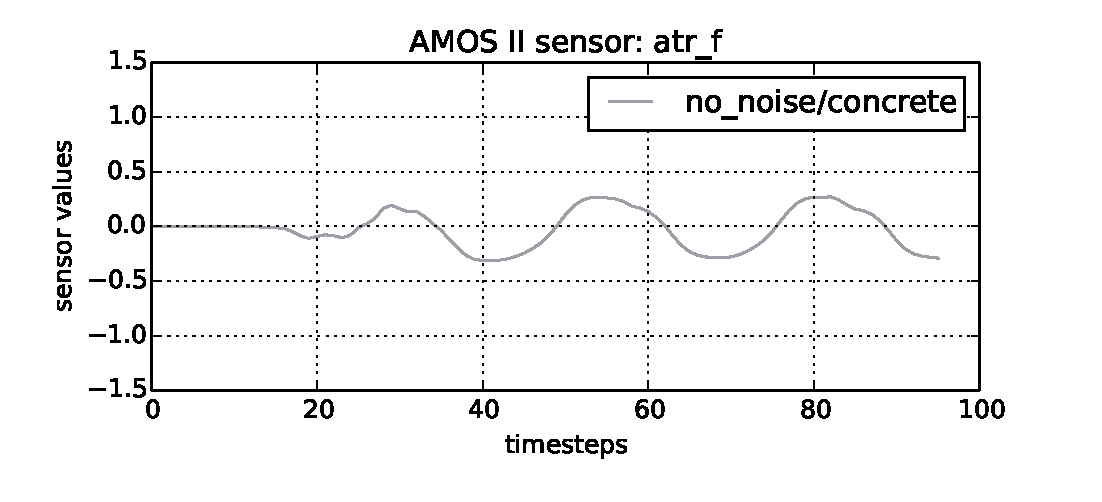
\includegraphics[width=1.0\textwidth]{plot_sensor_atr_f_nn_concrete.eps}
  \caption{Data example: ATRf, concrete, 10 seconds}
  \label{fig:data_example}
\end{figure}

The \textit{no\_noise} indication in the figure legend reffers to \cref{ssec:terrain_noise}. An optimal starndard deviation value of the additive Gaussian noise is not known. Therefore some data for several values of this parameter has been generated. The simulation has been gradually run for:

\begin{itemize}
\item $ \sigma_p = 0.0 $ (no noise)
\item $ \sigma_p = 0.01 $ (noise 1\%)
\item $ \sigma_p = 0.03 $ (noise 3\%)
\item $ \sigma_p = 0.05 $ (noise 5\%)
\item $ \sigma_p = 0.1 $ (noise 10\%)
\item $ \sigma_p = 0.2 $ (noise 20\%)
\end{itemize}

The $ \sigma_p $ is a standard deviation percentage, as shown in \cref{code:terrain_noise}, this $ \sigma_p $ is applied on qualities ranges and so corresponding standard deviation values $ \sigma_i $ are computed.

It is always recommended to store rough data before some processing, hence the simulator creates \textit{.txt} files of structure symbolized in \cref{txt:rough_data} (with the reference to sensors shortcuts in \cref{tab:proprioceptors}). 

\begin{lstlisting}[language=XML, caption={Rough sensory data files structure}, label=txt:rough_data]
timestep_001;ATRf;ATRm;ATRh;ATLf;...;FRh;FLf;FLm;FLh
timestep_002;ATRf;ATRm;ATRh;ATLf;...;FRh;FLf;FLm;FLh
...
timestep_100;ATRf;ATRm;ATRh;ATLf;...;FRh;FLf;FLm;FLh
\end{lstlisting}

There is a \textit{.txt} file of this structure for every single simulation run in the \textit{root/data/} directory (see \cref{app:code_documentation}).

All the data files are generated by a script called \textit{generate\_txt\_data.py} (\ref{app:code_documentation}). This script takes several arguments, like the number of jobs (simulation runs), terrain types involved or the terrain noise \textit{std} ($ \sigma_p $). Then a loop based on these parameters starts, where the simulation is launched and stopped after ten seconds each iteration. This is performed by calling a bash command (since the simulation is \textit{.cpp} based) and then killing the called process from python. The corresponding \textit{.txt} file is saved after each iteration by the simulation and then copied by the python script to a corresponding folder in \textit{root/data/}.

\begin{figure}[H]
  \centering
  \includegraphics[width=0.8\textwidth]{generating_data}
  \caption{The process of data acquisition from the simulation.}
  \label{img:generating_data}
\end{figure}

In this manner, \textit{.txt} files for all terrains and all mentioned $ \sigma_p $ are saved into a structure illustrated on \cref{img:data_dir_structure}. Each \textit{.txt} file contains approximately 100 lines, one for each simulation step (as shown in \cref{txt:rough_data}). Every line then contains values of the 24 proprioceptive sensors.

\begin{figure}[H]
  \centering
  \includegraphics[width=0.8\textwidth]{data_dir_structure}
  \caption{The structure of rough data directory.}
  \label{img:data_dir_structure}
\end{figure}

Right after the data generation, a script called \textit{clean\_txt\_data.py} (\ref{app:code_documentation}) is used to check the created \textit{.txt} files. As it takes a long time to generate all the data, sometimes the simulation fails and the files are incomplete. Hence the script checks whether there are enough timesteps (at least more than 95) and also if the steps are not messed. Files that fail during the inspection are removed. As \cref{img:data_dir_structure} reveals, there are \textbf{500} \textit{.txt} files for every \textit{noise/terrain} configuration. This allows creating datasets of 500 samples per class.

\section{Building a Feature Vector} \label{sec:feature_vector_compilation}
So far, the hexapod simulation has been introduced, virtual terrain types defined and the simulator has been run on these terrains and for various values of terrain noise power. All the data has been acquired from the simulation as \textit{.txt} files. Hence the simulation is not needed anymore and only the gathered data are used for the following processing.

Classification tasks are generally based on datasets consisting of samples and corresponding targets. The samples need to be represented in a numerical way in order to be processed by a computer and its appropriate algorithms. In machine learning, this numerical representation of an object is called \textit{a feature vector}, an n-dimensional vector of numerical values. This section is devoted to building a feature vector out of the data gathered from proprioceptive sensors.

This part of the process is crucial as the way of feature vector compilation can influence classification results a lot. Information loss or redundant structures are quite frequent mistakes here. Therefore, as the optimal structure is not known, several possibilities are tested again and therefore some new global process parameters appear at this point (mentioned already in \cref{sec:overall_process_summary}).

For this particular problem, the task is to form one feature vector out of the content of one \textit{.txt} file (got in \cref{sec:data_acquisition}), as each of these files contains data for one sample (see \cref{img:feature_vector_forming}).

\begin{figure}[H]
  \centering
  \includegraphics[width=1.0\textwidth]{feature_vector_forming}
  \caption{Forming a feature vector out of a data file.}
  \label{img:feature_vector_forming}
\end{figure}

At this point, one may ask for the reason of using several timesteps for creating one sample. It is assumed that a proper terrain classification using proprioceptors at one moment in time is at least difficult, if not impossible. Therefore the idea is to let the robot walk for a while and take down the dynamics of the sensors. Of course, the more timesteps are used for one sample, the more time the classification takes. Because of these arguments the number of timesteps is left as a global process parameter and it is a subject for later discussion.

Sensors selection defines another global parameter coming out of this section. The anticipation is that the feature vector becomes redundant using all of the 24 sensors, as many of them might behave similarly. However, for now all of them are used to show how the feature vector is built and it is also left for later discussion.

Parameters coming out of feature vector compilation and left for later discussion:
\begin{itemize}
\item number of timesteps used to build one feature vector (one sample)
\item sensors involved in classification
\end{itemize}

Now, with reference to \cref{img:feature_vector_forming}, the question is how to transform the \textbf{2D} data from \textit{.txt} files into \textbf{1D} vectors. The idea is to fix the \textit{timesteps} parameter and arrange the columns of the matrix into one vector. This implies having data from all sensors one by one next to each other and forming one feature vector together. 

In \cref{fig:sample_example} an example of this kind of forming is shown. For illustration there is just one terrain type (\textit{concrete}) involved. The number of timesteps is set to 40 and all 24 sensors are used, hence a feature vector of length 960 is gained. The corresponding sensors shortcuts (see \cref{tab:proprioceptors}) are added to the x-axis annotation. The 18 angle sensors are followed by the 6 foot contact sensors.

\begin{figure}[H]
  \centering
  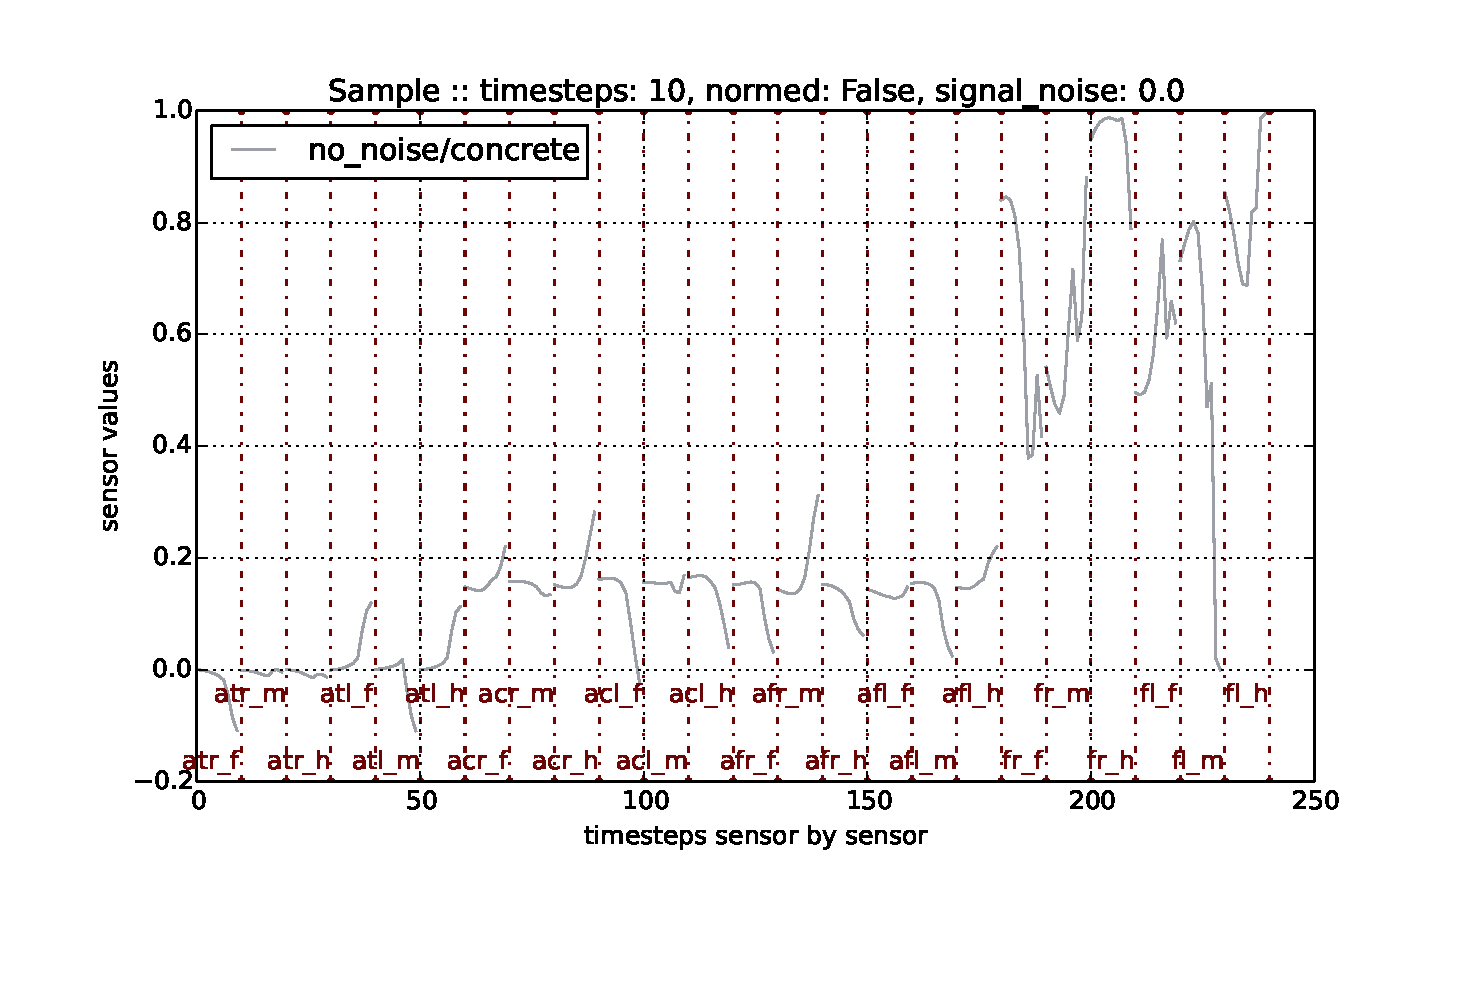
\includegraphics[width=1.0\textwidth]{sample_example.eps}
  \caption{Example of feature vector building.}
  \label{fig:sample_example}
\end{figure}

\subsection{Normalization} \label{ssec:normalization}
It is a good manner to keep the data normed - mapped to $ [0.0, 1.0] $ interval. The default range of foot contact sensors is already set to $ [0.0, 1.0] $, so there is nothing to change. For the angle sensors, the following approach is used to map the data. 

\begin{lstlisting}[language=Python, caption={Data normalization}, label=code:data_normalization]
def norm_signal(s, a_min, a_max):
  l = [min(max(float((x-a_min))/(a_max-a_min), 0), 1) for x in s]   
  return l
\end{lstlisting}

The bounds (\textit{a\_min} and \textit{a\_max} used in \cref{code:data_normalization}) are defined by default sensors ranges (listed in \cref{tab:proprioceptors}). Also a $ [0, 1] $ interval overflow checking is added and values are adjusted if needed. This is a cover for the case ranges from \cref{tab:proprioceptors} were not accurate. The following figure (\ref{fig:sample_example_normed}) shows a normed feature vector example. The influence of normalization on classification results is another subject for the discussion.

\begin{figure}[H]
  \centering
  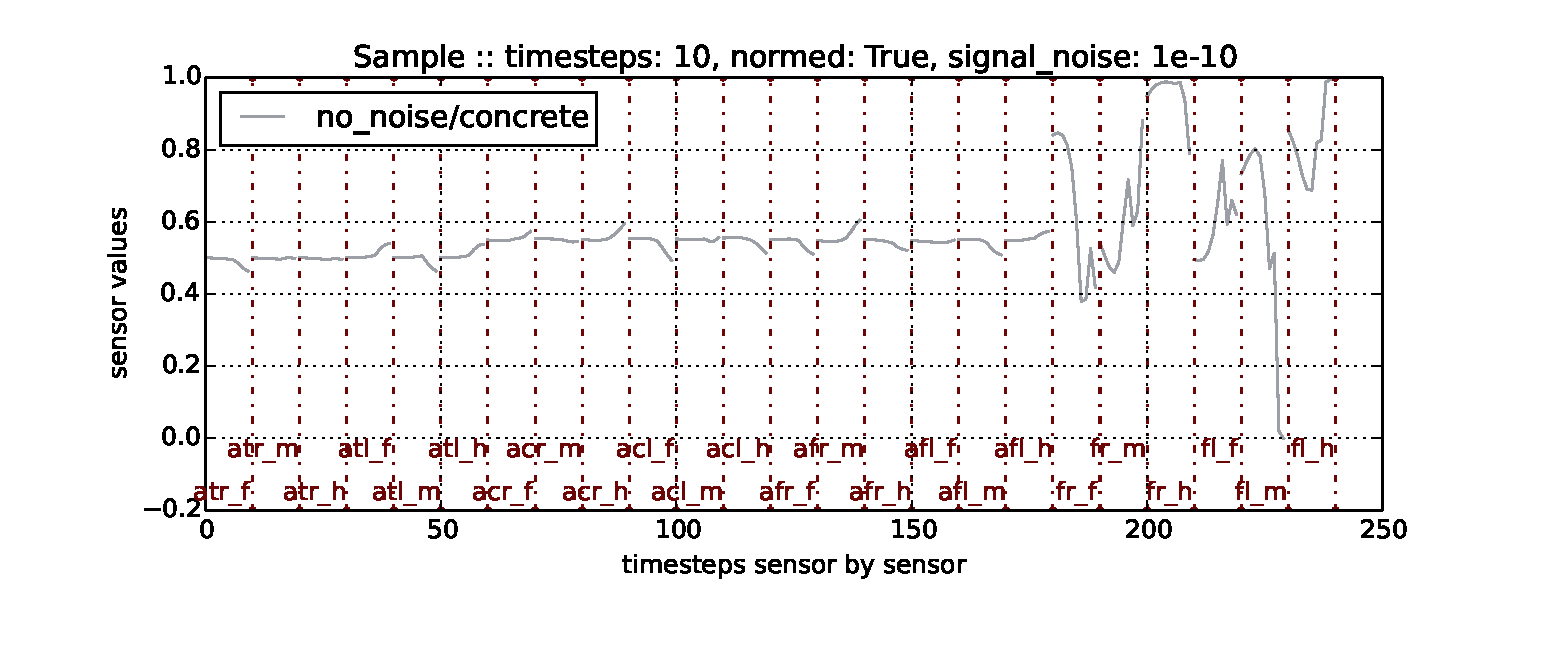
\includegraphics[width=1.0\textwidth]{sample_example_normed.eps}
  \caption{Example of feature vector - normed.}
  \label{fig:sample_example_normed}
\end{figure}

\subsection{Signal Noise} \label{ssec:signal_noise}
In \cref{ssec:terrain_noise} a few general reasons for noising simulation data are disscused. In that case an additive Gaussian noise is used to make the terrains definitions (from \cref{tab:terrains_parameters}) more complex.

For similar reasons a signal noise is added to the sensory data. In reality the mechanical sensors might shake, be influenced by environmental conditions or simply may not work as well as expected, while the data coming from the simulated sensors are always deterministic.

Right after the data normalization, a white Gaussian noise is added to the normed feature vectors. This time it is performed in Python, using the \textit{random.normal()} function of \textit{numpy} library to get the \textit{normal distribution} with zero mean (\cref{code:adding_signal_noise}).

\begin{lstlisting}[language=Python, caption={Adding signal noise in python}, label=code:adding_signal_noise]
def add_signal_noise(signal):
  noise = np.random.normal(loc=0, scale=STD, size=len(signal))
  return [x+n for x, n in zip(signal, noise)]
\end{lstlisting}

Also in this case, it is difficult to estimate an optimal signal noise power (STD in \cref{code:adding_signal_noise}). Therefore it is left as another global process parameter and its influence is discussed in the results part. It is defined as a percentage of the $ [0.0, 1.0] $ interval and as the signals are normed in advance, there is no need for another processing of this parameter.

\section{Datasets Creation} \label{sec:dataset_creation}
Reffering to \cref{img:terrain_classification_process}, in this section the \textit{create\_terrains\_dataset.py} script is introduced. At this part of the process all the data files are ready and also the form of feature vectors is determined. The task is to transform all the data into so called datasets.

There are usually three sets of data used for classification tasks - training, validation and testing data. These three sets must be disjunctive, meaning they cannot have a single element in common. All these three sets together form a dataset.

\begin{figure}[H]
  \centering
  \includegraphics[width=0.8\textwidth]{three_sets}
  \caption{Three sets of data in a dataset.}
  \label{img:three_sets}
\end{figure}

Each set of data consists of samples and targets (classes). The samples are represented by normed feature vectors (\cref{sec:feature_vector_compilation}) - lists of numerical floating point values from $ [0.0, 1.0] $ interval. The targets, in this case, match the names of virtually created terrain types (listed in \cref{tab:terrains_parameters}). Every sample must be uniformly assigned to precisely one target.

Once there are two ordered lists - a list of samples and a corresponding list of targets, these lists are split into the three sets shown in \cref{img:three_sets}. The script takes an argument called \textit{data\_split\_ratio} defining the proportions among the sets sizes. Defaultly the ratio is set to generate 80\% training, 10\% validation and 10\% of testing data.

\begin{figure}[H]
  \centering
  \includegraphics[width=0.8\textwidth]{create_dataset}
  \caption{\textit{create\_terrains\_dataset.py} : script workflow}
  \label{img:create_dataset}
\end{figure}

The workflow happening inside the \textit{create\_terrains\_dataset.py} script is illustrated in \cref{img:create_dataset}. During the overall process description in previous sections, some global process parameters have been collected. These configurations are now passed as arguments to this script and therefore several datasets of various properties can be generated.

The datasets files are saved in directory \textit{root/py/cache/datasets/amos\_terrains\_sim/} (see \ref{app:code_documentation}). Their structure is based on a powerful serializing and de-serializing Python algorithm implemented under a package called \textit{pickle (cPickle)}. On the same basis a package called \textit{shelve} is used to represent a dataset as a dictionary-link object. The files are saved with the \textit{.ds} suffix.

The list of all generated datasets can be found in \cref{app:list_of_datasets}. These datasets and influence of individual parameters are evaluated in the results section (\cref{chapter:06:experimental_evaluation}).

\section{Training and Classification}
Having a dataset enables to train a classifier, a machine learning tool that is able to learn some behavior on one part of some data (training and validation) and then perform similarly on another "never seen" part of the data (testing) - illustrated in \cref{img:three_sets}.

There are many classification methods differing in mathematical backgrounds and each of them has some pros and cons on various types of data. However, all of them have some general functionalities that comply with some kind of convention. For instance, there are at least two functions that every classifier should be capable of:

\begin{description}
\item[fit()] : Fitting some data to a model. This function usually takes training samples and their targets as arguments. Additiionally, it can take some validation data and/or learning parameters. Then a model is trained.
\item[predict()] : This function is then called when a model is already trained. It takes one or more samples of testing data and returns the predicted target(s).
\end{description}

This convention enables testing different classification approaches on the same data in the same way. Therefore also the implemented network library \textit{kitt\_nn} (see \cref{chapter:04:neural_net_implementation}) provides these functions and is capable of working with datasets of the same structure as the public \textit{.py} classifiers (discussed in sections \ref{ssec:sknn} and \ref{ssec:other_classifiers}).

In the overall process diagram (\cref{img:terrain_classification_process}) two scripts for training neural networks are included. The first one, \textit{kitt\_train.py}, uses the implemented network library \textit{kitt\_nn} (\cref{chapter:04:neural_net_implementation}) and the script called \textit{sknn\_train.py} uses a public library \textit{Scikit-neuralnetwork}, which is described in \cref{ssec:sknn}. It is important that these two scripts use the same workflow, which is illustrated in \cref{img:train_and_test_network}.

\begin{figure}[H]
  \centering
  \includegraphics[width=0.8\textwidth]{train_and_test_network}
  \caption{\textit{kitt\_train.py} and \textit{sknn\_train.py} : scripts workflow}
  \label{img:train_and_test_network}
\end{figure}

The scripts take several arguments (firstly listed in \cref{sec:overall_process_summary}) that differentiate the final trained networks and their performances. The first one is the dataset that the network is trained on. This parameter brings its own configuration (see its input parameters in \cref{img:create_dataset}) and so its setting parametrizes the classifier as well.

Next, one needs to define the network initial structure in sense of number of hidden layers and number of neurons in each of these layers. The input and output layers are determined by the dataset. There are many parameters to be defined for learning like \textit{batch size}, \textit{initial random state} etc. In this reasearch, only the learning rate and the number of epochs are used as training parameters. The learning process follows the implemented backpropagation algorithm described in \cref{sec:learning_algorithm}.

Finally, the trained network needs a file name, as it is saved the same way as the datasets (see \cref{sec:dataset_creation}) - using the \textit{pickle (cPickle)} package, just with the \textit{.net} suffix.

\subsection{Evaluation Methods} \label{ssec:evaluation_methods}
A trained network is evaluated on testing data. This evaluation provides a set of the most important classification metrics \citep{article:scikit-learn}.

\begin{description}
\item[accuracy] : the set of labels predicted for a sample must exactly match the corresponding set of true labels
\item[precision] : ability of the classifier not to label as positive a sample that is negative
\item[recall] : the ability of the classifier to find all the positive samples
\item[F1 score] is interpreted as a weighted average of the precision and recall, where an F1 score reaches its best value at 1 and worst score at 0. The relative contribution of precision and recall to the F1 score are equal. Formula:
\begin{equation}
F1 = \frac{2 * precision * recall}{precision + recall}
\end{equation}
\item[confusion matrix] : a confusion matrix $ C $ is such that $ C_{i, j} $ is equal to the number of observations known to be in group $ i $ but predicted to be in group $ j $.
\end{description}

\subsection{Terrain Classification using Pruned Nets} \label{ssec:pruned_net_on_terrains}
As the overall process diagram (\cref{img:terrain_classification_process}) shows, the developed network pruning algorithm (\cref{chapter:network_pruning_algorithm}) is tested on the terrain datasets. The approach has been already described. 

Evaluation in... \textbf{TODO:} describe the process here and reffer the results after they are gathered.


\subsection{Scikit-learn Neural Network Library} \label{ssec:sknn}
In order to verify the functionality of implemented neural network library (\cref{chapter:04:neural_net_implementation}), a provided public library is used. As the official description says \citep{misc:sknn}, this library implements multi-layer perceptrons as a wrapper for the powerful \textit{pylearn2} library that is compatible with \textit{scikit-learn} for a more user-friendly and Pythonic interface.

This step has been considered with the aim to test another implementation of the learning algorithm rather than to obtain better classification results. As the only learning parameters are the \textit{net structure}, the \textit{learning rate} and the \textit{number of epochs}, some other default parameters of the tested network are shown in \cref{code:sknn_net}.

\begin{lstlisting}[language=Python, caption={Sknn classifier specification \citep{misc:sknn}}, label=code:sknn_net]
class sknn.mlp.Classifier(layers, warning=None, parameters=None, 
random_state=None, learning_rule=u'sgd', learning_rate=0.01, 
learning_momentum=0.9, normalize=None, regularize=None, 
weight_decay=None, dropout_rate=None, batch_size=1, n_iter=None, 
n_stable=10, f_stable=0.001,  valid_set=None, valid_size=0.0, 
loss_type=None, callback=None, debug=False,  verbose=None)
\end{lstlisting}

\subsection{Searching for Optimal Configuration (Grid Search)} \label{ssec:grid_search}
\textbf{TODO :} describe here how the best parameters have been found using GridSearch

datasets implication -> nets based on nets params (learning rate and number of epochs), fixed batch size, number of stable iterations ....

\subsection{Other Classifiers} \label{ssec:other_classifiers}
\textbf{TODO :} describe here how other classifiers have been tested and reffer to the results part

SVM, k-NN, RandomForest